\documentclass{beamer}    
\mode<presentation> 
  \usetheme{Warsaw}       
  \usecolortheme{wolverine} 
  \setbeamercovered{transparent} 

\usepackage{beamerthemesplit}
\usepackage{amsmath,amssymb}
\usepackage[latin1]{inputenc}
\usepackage[english]{babel}
\usepackage{ragged2e}
\usepackage{multimedia}
\justifying
\title[\hspace{5cm}\textrm{\LaTeX}]{Evolutionary Dynamics: Fitness, Cooperation and Gene Expression Noise.}
\author[Alejandro Mahecha]{Alejandro Mahecha}
\institute{Universidad de los Andes\\ Departamento de F�sica\\ Grupo de Biof�sica}
\setbeamertemplate{bibliography item}[text]
\begin{document}
\frame{\titlepage}
\section*{Outline}
\frame{
\tableofcontents}
\section[Natural Selection and Fitness]{Natural Selection and Fitness}
\frame{
\frametitle{Natural Selection and Fitness}
What evolution is?
\begin{itemize}
\item Today in colloquial language evolution means, changes over time. From it can be inferred that evolution happens in many things around us: changes in the shapes of mounts, the different leafs of trees across seasons, etc, but evolution in living systems has a key difference, reproduction.
\item Biological evolution is changes in the characteristics of populations of organisms over the course of generations. Where these changes are inherited.
\end{itemize}
}

\frame{
Which are the mechanisms that leads to an evolutionary process?.
Evolutionary dynamics have three basic mechanisms:
\begin{itemize}
\item Replication.
\item Mutation: mistakes in genetic replication. Is responsible for generating different types. 
\item Selection.
\end{itemize}
}
\frame{
\begin{figure}
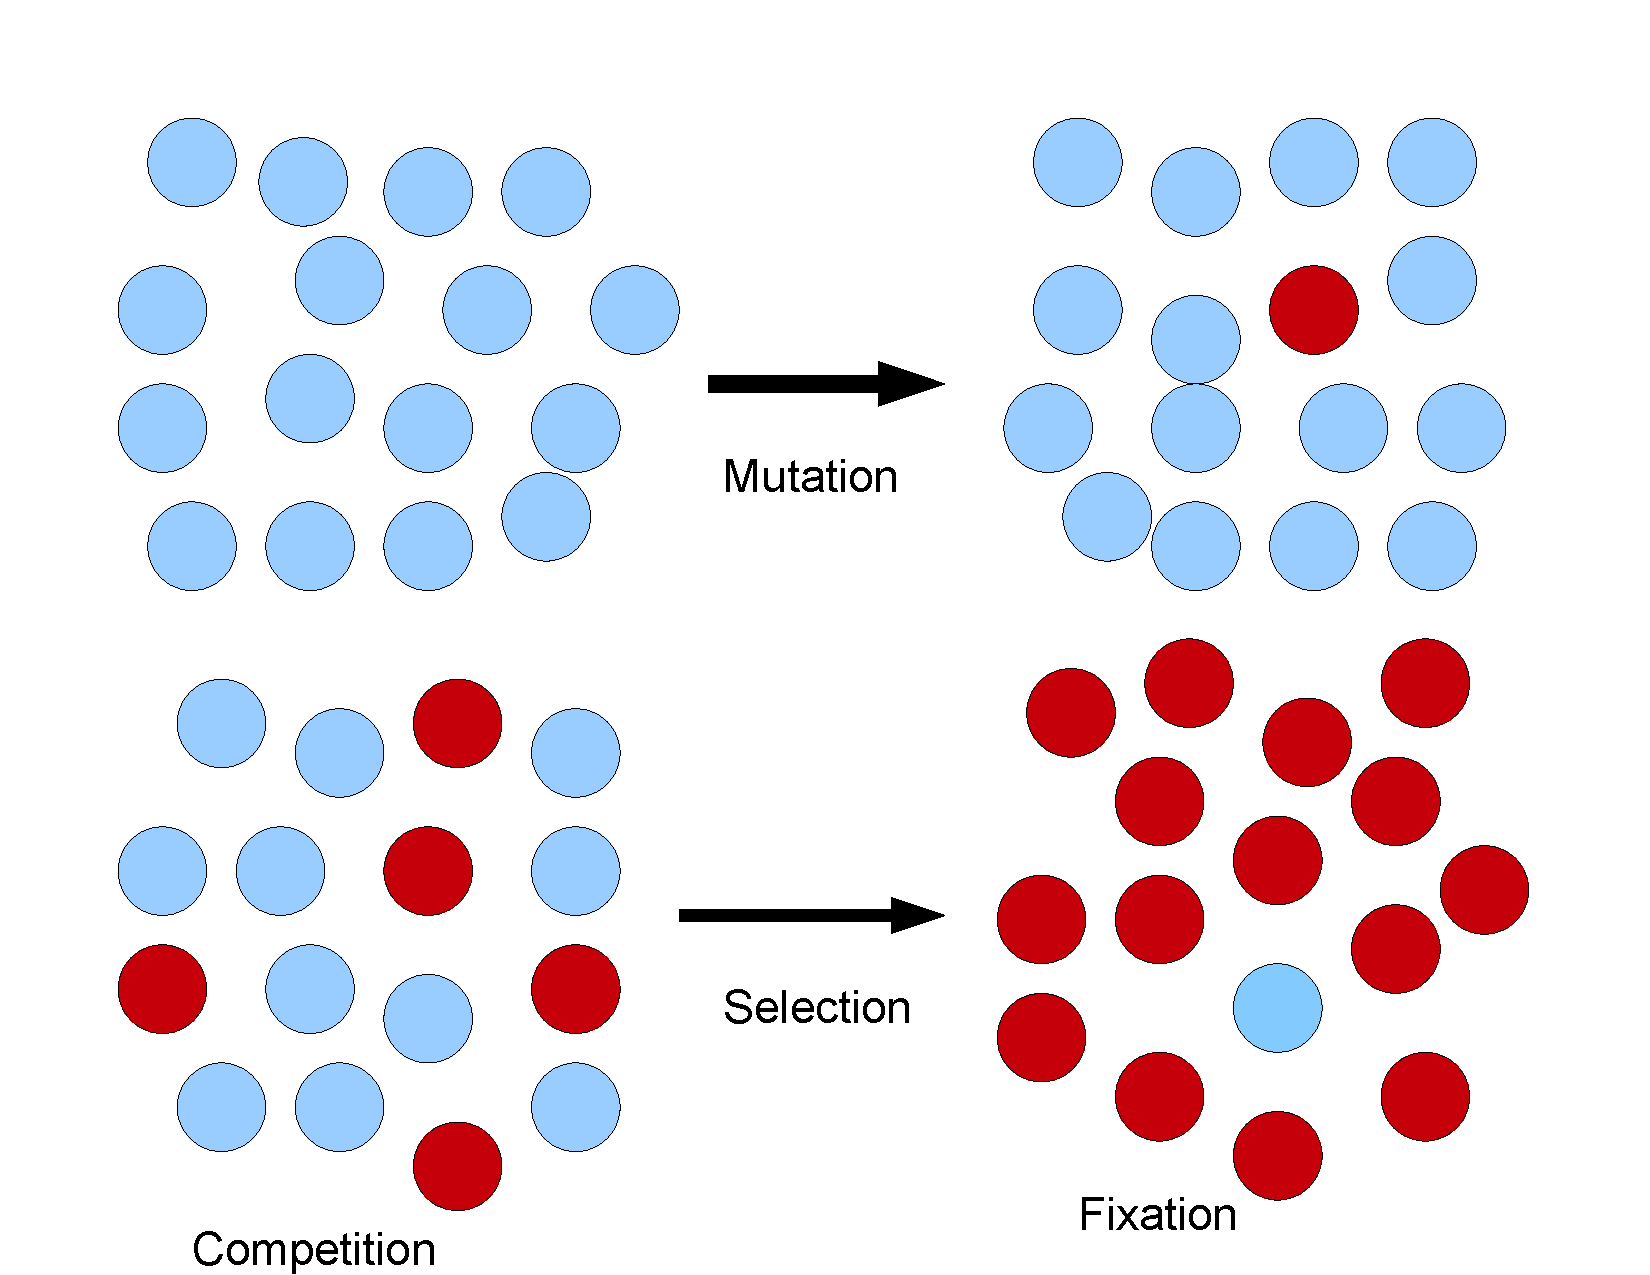
\includegraphics[width=6cm,height=5cm]{naturalselection.pdf}
\end{figure}
}


%\begin{figure}
%\includegraphics[width=6cm,height=5cm]{microcanales}
%\end{figure}


\frame{

\begin{columns}[c]
\column{2in}
\begin{figure}
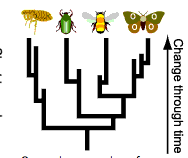
\includegraphics[width=4cm,height=4cm]{evolution.png}
\caption{www.evolution.berkeley.edu}
\end{figure}
\column{2in}
\begin{figure}
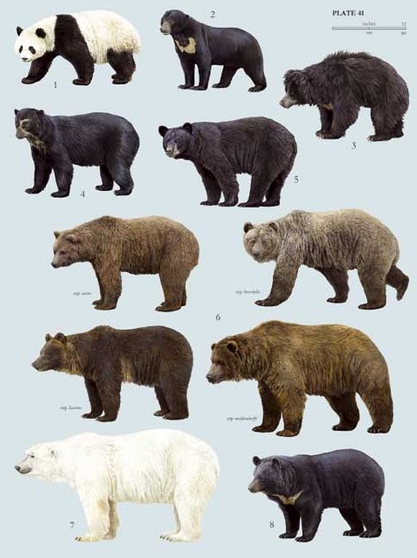
\includegraphics[width=4cm,height=4cm]{osos.png}
\caption{\url{http://images.yuku.com.s3.amazonaws.com/image/jpg/03616d619a16fb3ae47432d6694ed9f29153ac22_r.jpg}}
\end{figure}
\end{columns}
}
\frame{
Changes in traits across successive generations is the beginning of the way to explain the diversification in living beings.
\begin{figure}
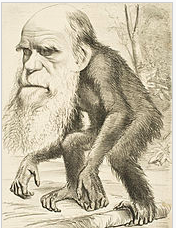
\includegraphics[width=2cm,height=2cm]{darwin.png}
\end{figure}
Darwin proposed Natural selection.
}
\frame{
Changes in population traits are gradual directional to the fittest trait, and through genetic inheritance the fittest characteristic gets fixed in the population depending on the environment.
\begin{figure}
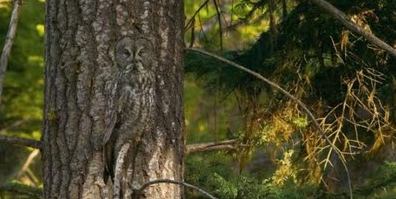
\includegraphics[width=6cm,height=4cm]{buo.png}
\end{figure}
}
\frame{
\begin{itemize}
 \item In the early 20th century scientist created approaches to modeling natural selection mathematically.
 \item A quantity that makes a characteristic more selective than others.
 \item This quantity is called fitness.
 \end{itemize}
}
\frame{
Fitness is usually defined as the average number of offsprings produced by individuals of a certain type and the average number of these that survive.
\begin{figure}
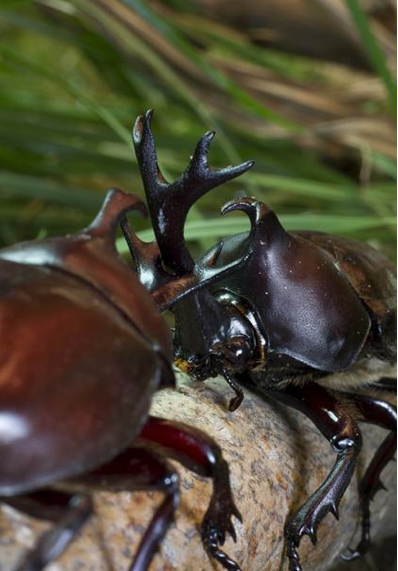
\includegraphics[width=5cm,height=4cm]{escarabajo.png}
\end{figure}
}
\frame{
The per capita growth rate $R$ of a genotype.
\begin{figure}
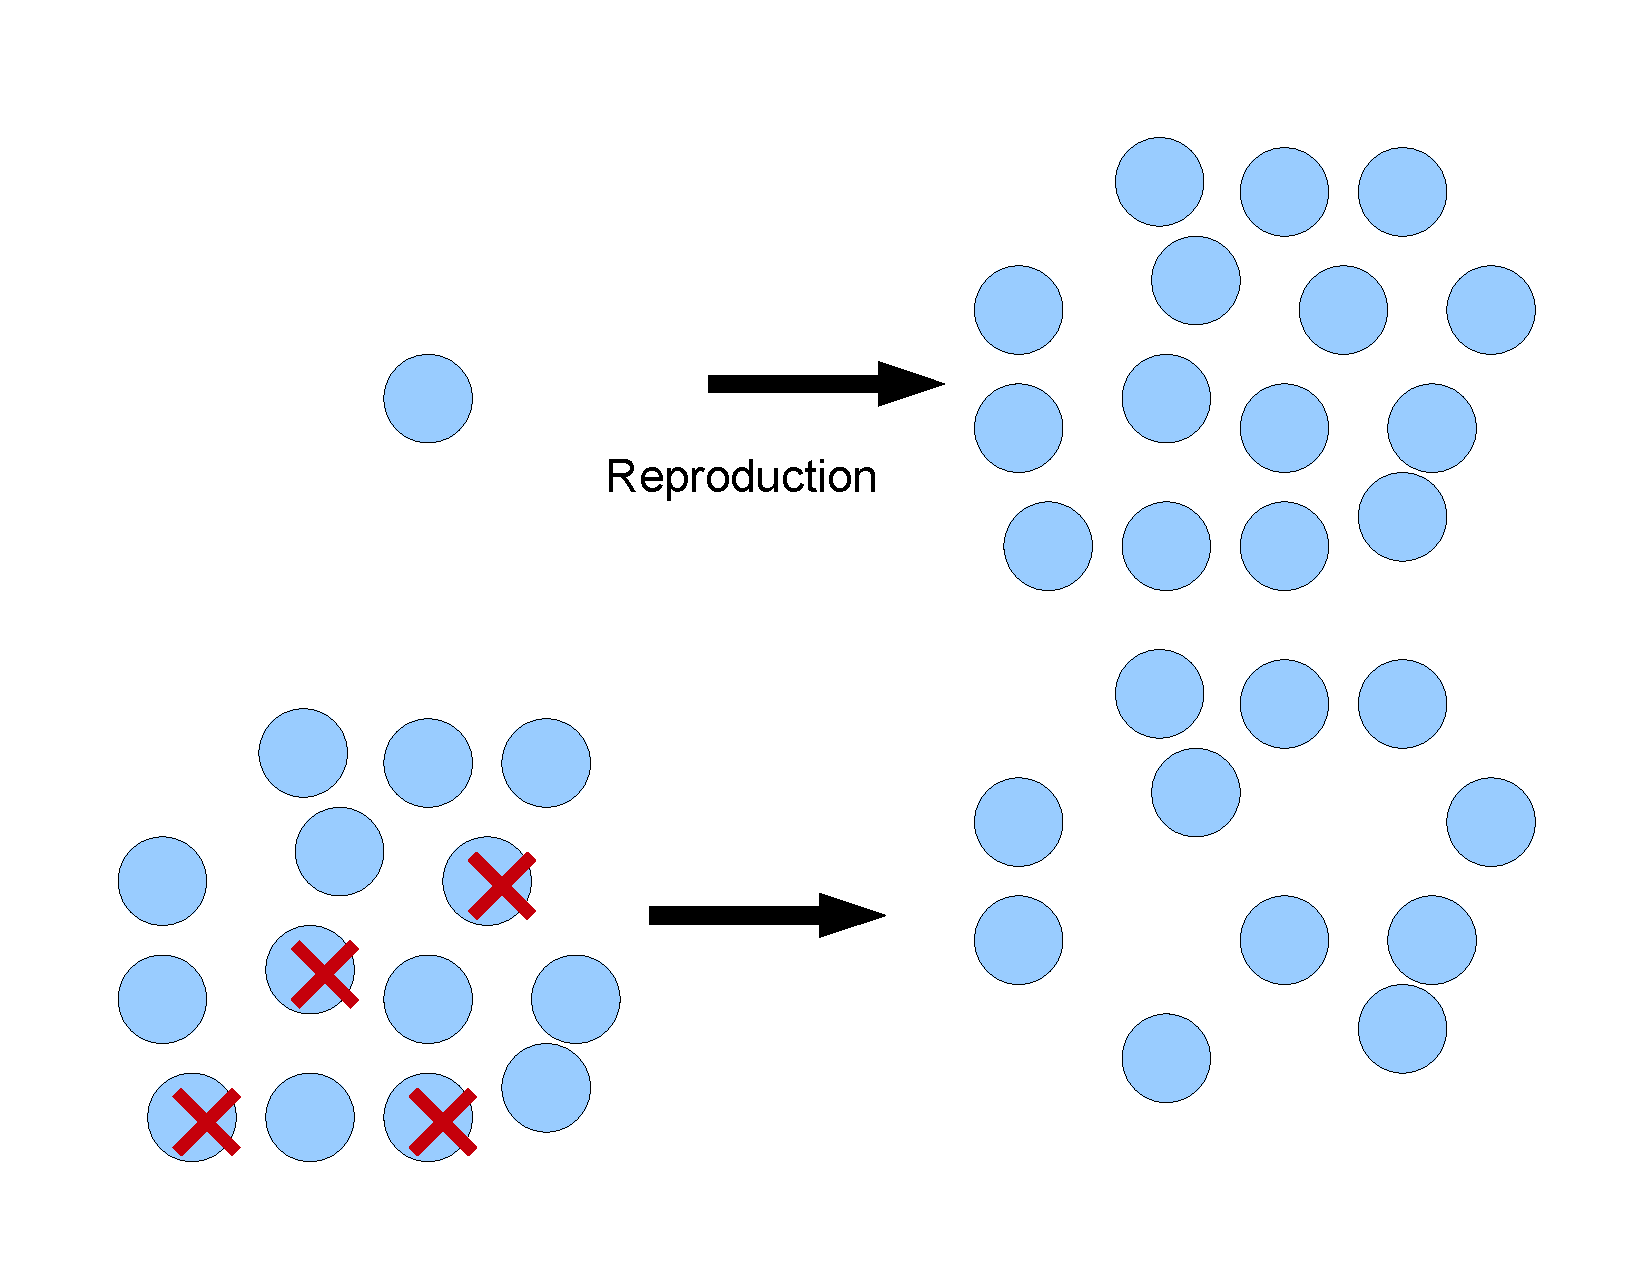
\includegraphics[width=5cm,height=4cm]{percapita.pdf}
\end{figure}
Fitness$=$(proportion surviving)x(average fecundity). Suppose that an organism lays an average of $60$ eggs, and $0.05$ of then survive to reproductive age. $f=0.05\times60=3$. 
}
\frame{
Because our constant population $N$ simulation and usually in stochastic model for evolution, fitness is just the reproductive contribution of each individual of a certain type. The death rate is due to the $N$ constant size.
 \begin{figure}
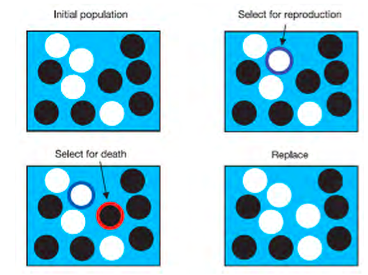
\includegraphics[width=5cm,height=3.5cm]{simulation.png}
\end{figure}
$f_{i}=offsprings/time$ in our simulation with asexual reproduction.
}
\frame{
Fitness is not just due to physical advantages, it have been seen that it also due to social behaviors and altruistic interactions.
  \begin{columns}[c]
 \column{2in}
 \framebox{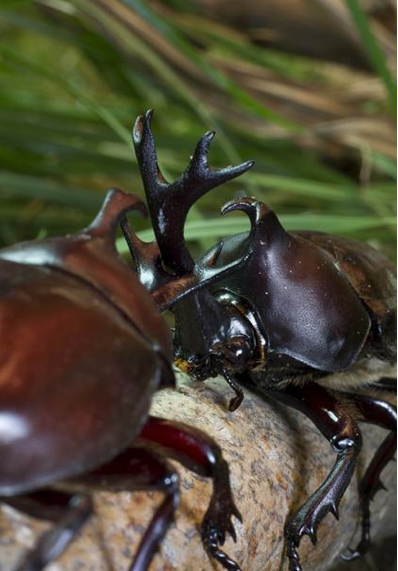
\includegraphics[width=2in,height=1.5in]{escarabajo.png}} 
\column{2in} 
 \framebox{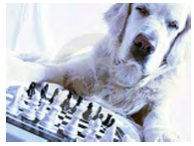
\includegraphics[width=2in,height=1.5in]{perro.png}} 

\end{columns}

}
\section[Deterministic Model of Reproduction and Selection]{Deterministic Model of Reproduction and Selection}
\frame{
\frametitle{Deterministic Model of Reproduction and Selection}
Bacterial cells in a perfect environment.
\begin{equation}
x_{t+1}=2x_{t} \;\;\; x_{t}=x_{0}2^{t}
\end{equation}
Differential equation for exponential growth at rate $r$. Where the time of cell division is an exponential distribution with average $1/r$.
\begin{equation}
\dot x=rx \;\;\; x(t)=x_{0}e^{rt}.
\end{equation} 
\begin{equation}
\frac{dN(t)}{dt}=rN(t)-dN(t)-mN(t).
\end{equation}
}
\frame{
Suppose we have two organism $A$ and $B$ competing, with fitnesses $f_{A}$ and $f_{B}$ , frequencies $x_A$ and $x_B$ and size $N$.
 \begin{equation}
 \frac{dx_A}{dt} =f_A x_{A} - \phi,
 \end{equation}  
  \begin{equation}
 \frac{dx_B}{dt} =f_B x_{B} - \phi.
 \end{equation}  
 \begin{equation}
\frac{dx_{A}}{dt}=x_{A}(1-\frac{x_{A}}{N})(f_{A}-f_{B}).
 \end{equation} 
}
\frame{
\begin{equation}
x_{A}(t)=\frac{x_{A0}e^{(f_{A}-f_{B})t}}{1-\frac{x_{A0}}{N}+\frac{x_{A0}}{N}e^{(f_{A}-f_{B})t}}.
\end{equation}  
\begin{columns}[c]
 \column{1.5in}
 \framebox{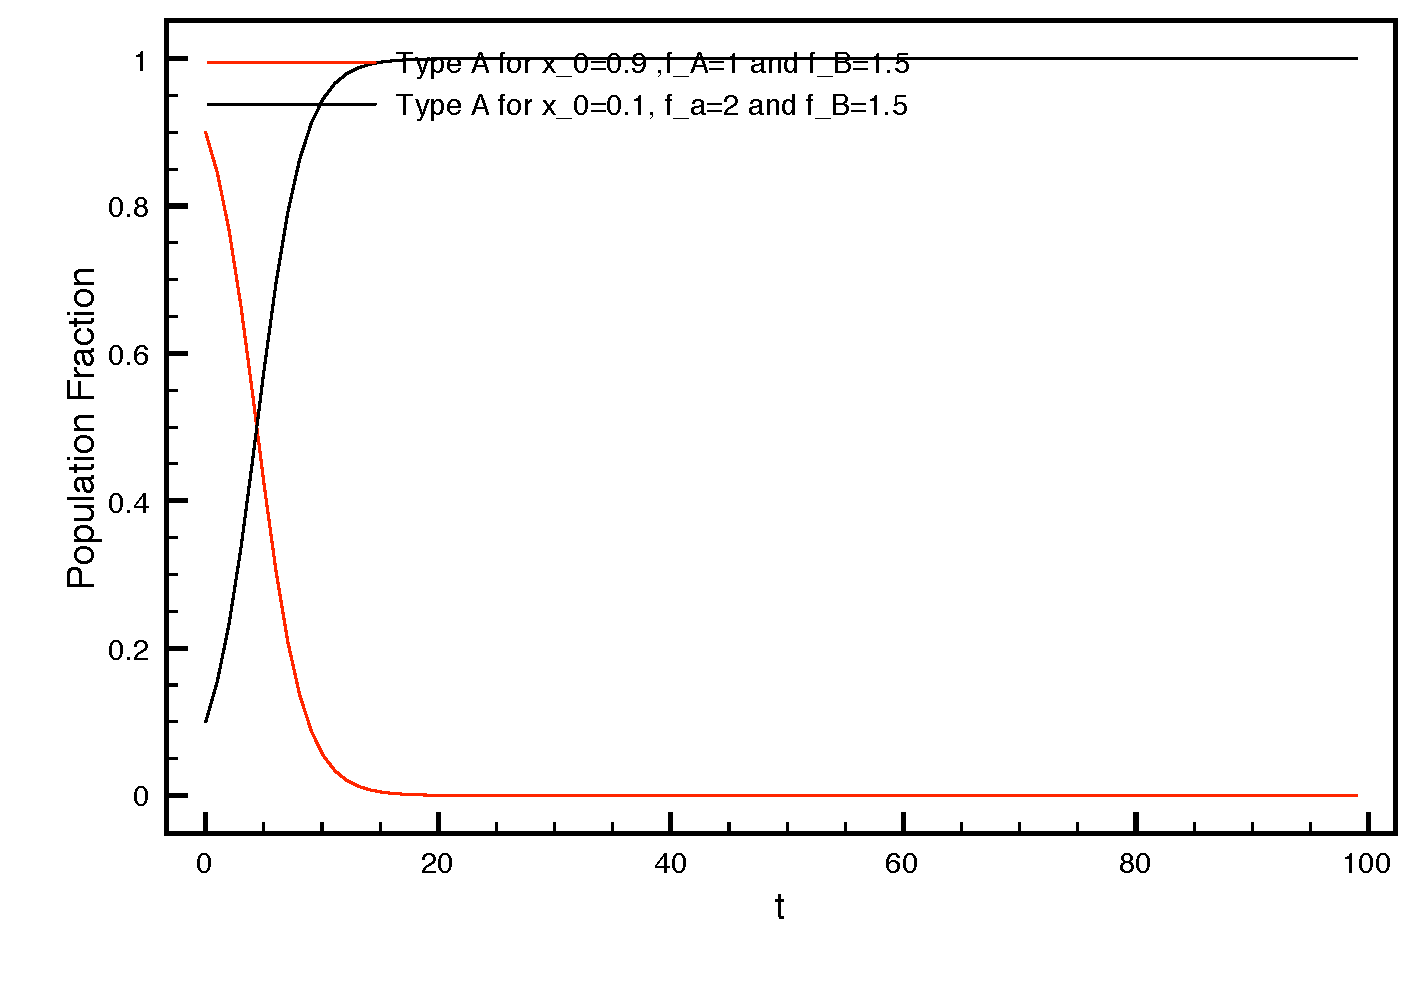
\includegraphics[width=2in,height=1.5in]{DeterministicSelection.pdf}} 
\column{2in} 
\framebox{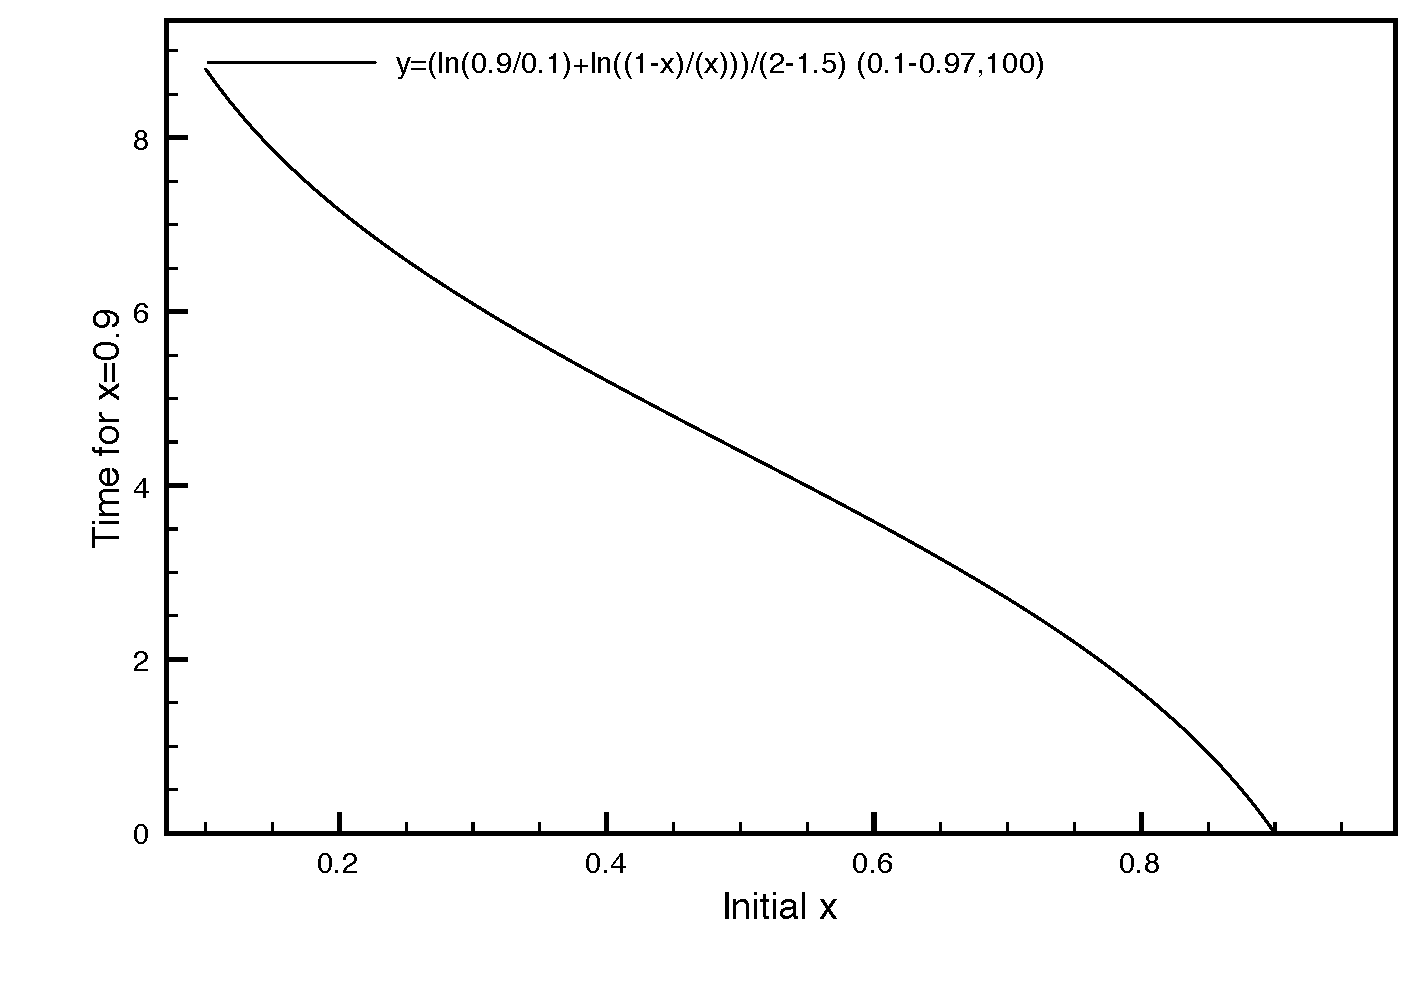
\includegraphics[width=2in,height=1.5in]{DominanceTimeVsInitialx.pdf}}
\end{columns}
}

\section[Markov Chain and Moran Process]{Markov Chain and Moran Process}
\frame{
\frametitle{Markov Chain and Moran Process}
\begin{figure}
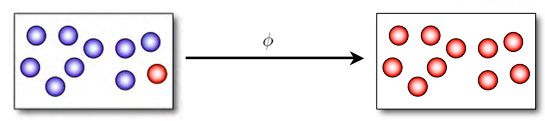
\includegraphics[width=7cm,height=2cm]{pasodiscreto.png}
\end{figure}
\begin{figure}
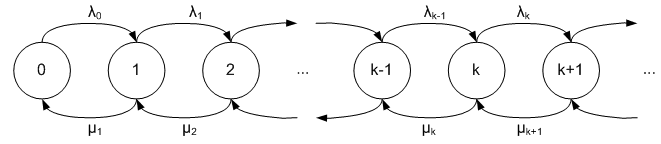
\includegraphics[width=7cm,height=2cm]{markovchain.png}
\end{figure}
\begin{figure}
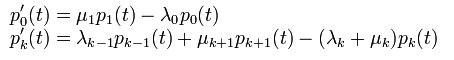
\includegraphics[width=6cm,height=1cm]{masterequation.png}
\end{figure}
}
\frame{
\frametitle{Moran Process}
\begin{figure}
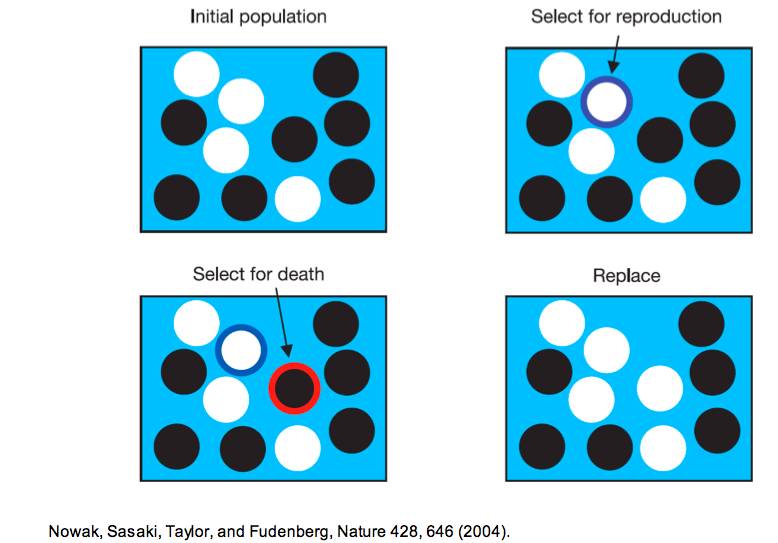
\includegraphics[width=6cm,height=4cm]{moranprocess.png}
\end{figure}
}
\frame{
\frametitle{Moran Process Simulation}
Two types with fitness $r$ and $s$. At each time step one types i selected for reproduction with probability
\begin{equation}
\frac{ri}{ri+s(n-i)}
\end{equation}
Then one individual is replaced randomly  with the new offspring.
\begin{equation}
\frac{i}{n}\;\; , \;\; \frac{n-i}{n}
\end{equation}
}
\frame{
Transition probabilities
\begin{equation}
\begin{split}
P_{i,i+1}&=\frac{ri}{ri+s(n-i)}\frac{n-i}{n}\\
P_{i,i-1}&=\frac{s(n-i)}{ri+s(n-i)}\frac{i}{n}
\end{split}
\end{equation}
The master equation for this system is:
{\tiny
\begin{equation}
\frac{dP_{i}}{dt}=-(\frac{ri}{ir+s(n-i)}\frac{n-i}{n}+\frac{s(n-i)}{ir+s(n-i)}\frac{i}{n})P_{i}(t) + \frac{r(i-1)}{(i-1)r+(n-i+1)s}\frac{n-i+1}{n} P_{i-1}+ \frac{r(i+1)}{(i+1)r+(n-i-1)s}\frac{i+1}{n} P_{i+1}
\end{equation}
}
}
\frame{
The conditions for fixation probabilities $\rho_{i}$ are $\rho_{0}=0$, $\rho_{n}=1$ and
\begin{equation}
\rho_{i}=p_{i,i}\rho_{i}+p_{i,i+1}\rho_{i+1}+p_{i,i-1}\rho_{i-1}.
\end{equation}
Fixation time $\rho_{i}^{n}(t)$:
\begin{figure}
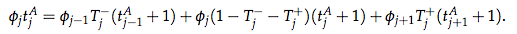
\includegraphics[width=8cm,height=0.7cm]{fixationTime.png}
\end{figure}

}
\frame{
%\url{http://tex.stackexchange.com/}\\
  %\href{http://www.nature.com/nature/journal/v436/n7049/extref/nature03831-s3.mpg}{Video Dielectroforecis, concentrador de c�lulas}
  \frametitle{Neutral Drift}
\begin{columns}[c]
 \column{2in}
 \framebox{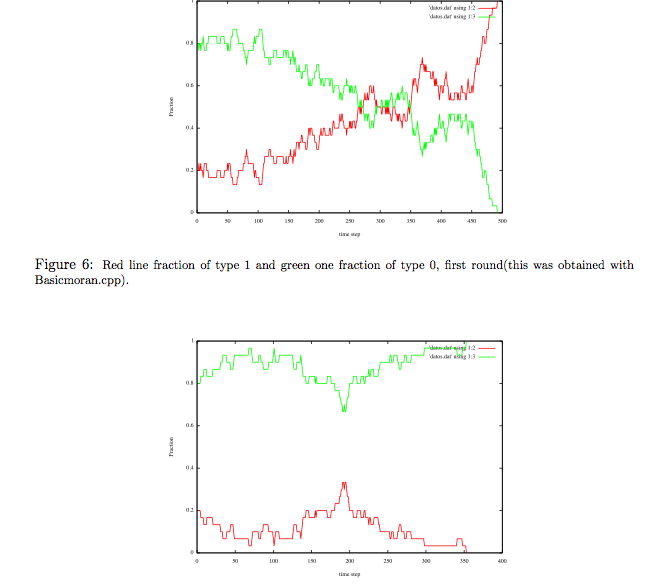
\includegraphics[width=2in]{neutraldrift.png}} 
\column{1.5in} 
$\rho_{i}=\frac{i}{n}$
 \end{columns}
}
\frame{
\begin{equation}
\rho_i = \frac{1-1/r^i}{1-1/r^n}.
\end{equation}
\begin{figure}
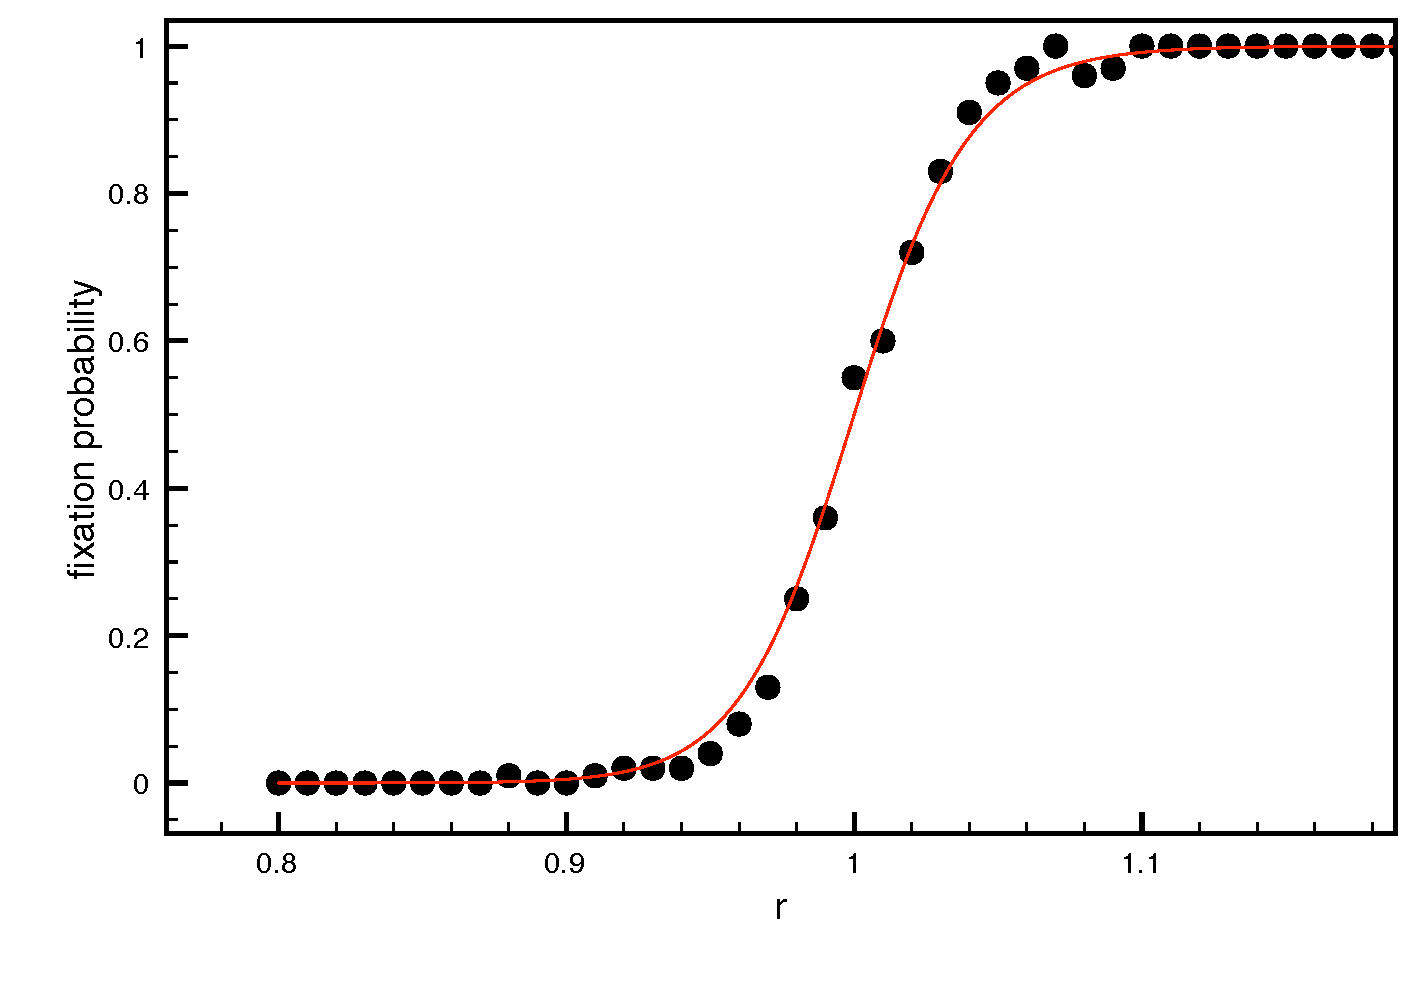
\includegraphics[width=6cm,height=5cm]{plot.pdf}
\end{figure}
}
\section[Game Theory, Cooperation and Fitness]{Game Theory, Cooperation and Fitness}
\frame{
\frametitle{Game Theory, Cooperation and Fitness}
Cooperate or cheating. They can be transfer to the next generation.
\begin{equation}
\bordermatrix{~ & C & D \cr
             C & R & S \cr
              D & T & P \cr}
\end{equation}
\begin{equation}
P_{C}=\frac{R(x-1)+S(N-x)}{N-1}
\end{equation} 
\begin{equation}
P_{D}=\frac{Tx+P(N-x-1)}{N-1}
\end{equation}
%\begin{figure}
%\includegraphics[width=6cm,height=5cm]{mecanica}
%\end{figure}
fitness as function of the payoff.
\begin{equation}
f_{C}=1-w+wP_{C} \;\;\; f_{D}=1-w+wP_{D}
\end{equation}
where $w$ is the intensity of selection.
}
\frame{
Selection is also at level of groups of the fittest individuals, which will reproduce faster. There is a Moran Process for GOUP SELECTION.
\begin{figure}
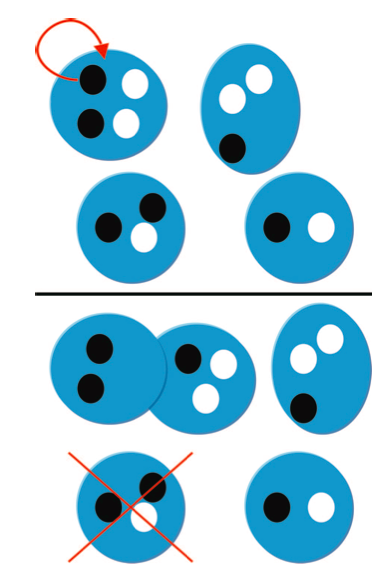
\includegraphics[width=6cm,height=6cm]{groupselection.png}
\end{figure}
}
\section{Stochastic Fitness}
\frame{
Due to internal noise, fitness is not deterministic.
\begin{figure}
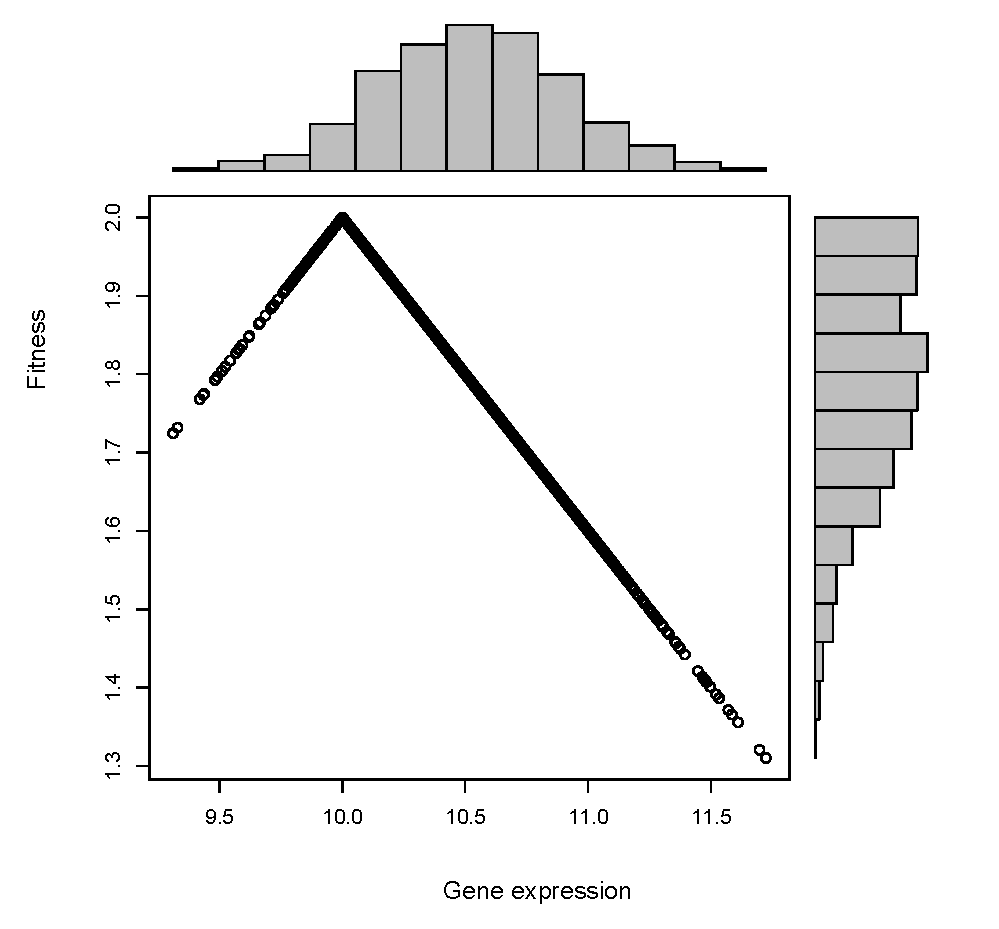
\includegraphics[width=6cm,height=6cm]{triangularfunctionHistogram.pdf}
\end{figure}
}
\frame{
\begin{equation}
p_{reproduction}=\frac{\sum_{i=1}^{n}f_{1i}}{\sum_{i=1}^{n}f_{1i} + \sum_{j=1}^{N-n}f_{0j}}
\end{equation} 
\begin{equation}
\rho_1=\left(1 + \sum\limits_{i=2}^{N}{\frac{(i-1)!(N-i)!}{(N-1)!}\prod\limits_{j=2}^{i}{\frac{\sum\limits_{m=1}^{N-(j-1)}s_m}{\sum\limits_{m=1}^{j-1}r_m}}}\right)^{-1}
\end{equation}
}
\begin{frame}[allowframebreaks]{Bibliography}
\bibliographystyle{plain}
\bibliography{cooperation}
\end{frame}
\end{document}
